% !TEX encoding = UTF-8
% !TEX TS-program = pdflatex
% !TEX root = ../tesi.tex

%**************************************************************
\chapter{Flussi conversazionali prodotti}
\label{cap:flussi di conversazione}
%**************************************************************

\intro{In questo capitolo verrà descritto il lavoro che è stato fatto di analisi, progettazione e implementazione dei flussi conversazioniali per Azzurra creati durante lo stage.}\\

%**************************************************************
\section{Analisi dei requisiti}
\subsection{Descrizione del problema}
Durante lo stage è stato deciso, in comune accordo con il tutor aziendale, di costruire due flussi conversazionali per il \g{bot} Azzurra, nello specifico:
\begin{itemize}
	\item \textbf{DeskBooking}: Questo flusso conversazionale consiste nel gestire le prenotazioni di un posto a sedere. Deve esserci la possibilità di richiedere una nuova prenotazione, visualizzare la lista delle proprie prenotazioni ed infine, scannerrizzare un \g{QR code} messo nel posto a sedere, per controllare se il lavoratore può usufruire e riscattare tale posto. C'è quindi bisogno di integrare un lettore di \g{QR code} in Azzurra per poter fare il controllo che consiste nell'aprire la fotocamera e scannerizzare il \g{QR code} che verrà usato per il controllo ed infine comunicare l'esito della verifica al lavoratore;
	\item \textbf{Planning}: Questo flusso conversazionale consiste nel far visualizzare al lavoratore il lavoro che deve svolgere. Deve esserci la possibilità di richiedere la visualizzazione del lavoro pianificato di uno specifico giorno oppure la possibilità di vedere il lavoro pianificato per tutta la settimana.
\end{itemize}
\subsection{Requisiti}
Ogni requisito sarà strutturato come segue:
\begin{itemize}
	\item Identificativo: \textbf{R[Importanza][Tipologia][Codice]}\\
	Dove:
	\begin{itemize}
		\item \textbf{Importanza:}
		\begin{itemize}
			\item \textbf{1}: Requisito obbligatorio, vincolante in quanto primario e fondamentale;
			\item \textbf{2}: Requisito desiderabile, non strettamente necessario ma che porta valore aggiunto riconoscibile;
			\item \textbf{3}: Requisito opzionale, relativamente utile.
		\end{itemize}
		\item \textbf{Tipologia:}
		\begin{itemize}
			\item \textbf{F}: Funzionale, definisce una funzione di un sistema di uno o più dei suoi componenti;
			\item \textbf{Q}: Qualitativo, definisce un requisito per garantire la qualità per un certo aspetto del prodotto;
			\item \textbf{P}: Prestazionale, definisce un requisito che garantisce efficienza prestazionale nel prodotto;
			\item \textbf{V}: Vincolo, definisce un requisito volto a far rispettare un dato vincolo.
		\end{itemize}
		\item \textbf{Codice:} Viene utilizzato per identificare univocamente il requisito tramite un numero progressivo.\\
	\end{itemize}
\end{itemize}
Dopo un’analisi del problema sono stati individuati i seguenti requisiti
\begin{table}[h]%
	\rowcolors{2}{grigetto}{white}
		\renewcommand{\arraystretch}{1.5}
	\centering
	\begin{tabularx}{\textwidth}{c X}
		\hline	
		\rowcolor{heavenly}
		\intest{Codice} &  \intest{Descrizione} \\	
		\hline			
		R1F1 & Il lavoratore deve poter accedere alla funzionalità di "Prenotazione posto".\\
		R1F2 & Il lavoratore deve poter inserire una nuova prenotazione di un posto a sedere.\\
		R1F3 & Il lavoratore deve poter visualizzare le sue prenotazioni.\\
		R1F4 & Il lavoratore deve poter scansionare il \g{QR code} per poter usufruire del posto prenotato.\\
		R1F5 & Il lavoratore deve poter inserire la data in cui vuole prenotare il posto a sedere se disponibile.\\
		R1F6 & Il lavoratore deve poter inserire l'ora di inizio della prenotazione desiderata.\\
		R1F7 & Il lavoratore deve poter inserire l'ora in cui finisce la prenotazione desiderata.\\
		R1F8 & Il lavoratore deve poter inserire la stanza del posto a sedere che desidera prenotare.\\
		R1F9 & Il lavoratore deve poter inserire il posto a sedere che desidera prenotare se disponibile.\\
		R1F10 & Il lavoratore deve poter visualizzare il messaggio di conferma se la prenotazione del posto a sedere è andata a buon fine.\\
		R1F11 & Il lavoratore deve poter visualizzare il messaggio d'errore se non è stato possibile inserire la nuova prenotazione.\\
		R1F12 & Il lavoratore deve poter visualizzare le sue prenotazioni del giorno corrente.\\
		R1F13 & Il lavoratore deve poter visualizzare le sue prenotazioni del giorno successivo.\\
		R1F14 & Il lavoratore deve poter visualizzare le sue prenotazioni di uno specifico giorno.\\
		R1F15 & Il lavoratore deve poter inserire la data del giorno in cui vuole vedere le prenotazioni.\\
		\hline	
	\end{tabularx} \hbox{}
	\caption{Tabella del tracciamento dei requisiti}
\end{table}%


\begin{table}[h]%
	\rowcolors{2}{grigetto}{white}
		\renewcommand{\arraystretch}{1.5}
	\centering
	\begin{tabularx}{\textwidth}{c X}
		\hline		
		\rowcolor{heavenly}
		\intest{Codice} &  \intest{Descrizione} \\	
		\hline
		R1F16 & Il lavoratore, per ogni prenotazione, deve poter visualizzare l'ora di inizio della prenotazione.\\
		R1F17 & Il lavoratore, per ogni prenotazione, deve poter visualizzare l'ora in cui finisce la prenotazione.\\		
		R1F18 & Il lavoratore, per ogni prenotazione, deve poter visualizzare la stanza della prenotazione.\\
		R1F19 & Il lavoratore, per ogni prenotazione, deve poter visualizzare il posto della prenotazione.\\	
		R1F20 & Il lavoratore, dopo avere scannerizzato il \g{QR code} del posto a sedere, deve ricevere un messaggio di conferma che lo informa che può usufruire del posto a sedere.\\
		R1F21 & Il lavoratore, dopo avere scannerizzato il \g{QR code} del posto a sedere, deve ricevere un messaggio d'errore che lo informa che non può usufruire del posto a sedere.\\
		R1F22 & Il lavoratore deve poter visualizzazione la pianificazione di uno specifico giorno.\\
		R1F23 & Il lavoratore deve poter visualizzazione la pianificazione della settimana corrente.\\
		R1F24 & Il lavoratore deve poter inserire la data del giorno in cui vuole vederne la pianificazione del lavoro a lui assegnato.\\
		R1F25 & Il lavoratore deve poter visualizzare la data del giorno del lavoro pianificato.\\
		R1F26 & Il lavoratore deve poter visualizzare l'ora d'inizio del lavoro pianificato.\\
		R1F27 & Il lavoratore deve poter visualizzare l'ora in cui termina il lavoro pianificato.\\
		R1F28 & Il lavoratore deve poter visualizzare il lavoro che è stato pianificato per essere svolto.\\
		R1V1 & Per implementare i flussi conversazionali devono essere usati Angular e Ionic.\\
		R1V2 & Per gestire la fotocamera per la lettura del \g{QR code} deve essere usato il \emph{plugin} di Cordova, QR Scanner.\\
		\hline	
	\end{tabularx} \hbox{}
	\caption{Tabella del tracciamento dei requisiti}
\end{table}%
\clearpage
\section{Progettazione}
Dopo aver individuato i requisiti che descrivono i flussi da costruire, sono passato alla progettazione dei flussi. Come spiegato nel capitolo precedente i flussi conversazionali sono un insieme di blocchi che svolgono determinate funzioni a seconda del tipo di appartenenza. Grazie a ciò, la progettazione dei due flussi è iniziata con l'inserimento dei blocchi corretti e il collegamento tra di essi, ottenendo così due diagrammi che rappresentano i due flussi dove vengono visualizzati quali passi deve fare il \g{bot} Azzurra durante la conversazione con l'utente umano. Successivamente ho progettato i metodi da aggiungere a quelli esistenti per poter creare i messaggi nel modo corretto.\\
Di seguito vengono illustrati i diagrammi dei flussi fatti.

\subsection{Gestione delle prenotazioni dei posti}
Nei seguenti diagrammi viene visualizzato l'insieme dei blocchi che fanno parte del flusso conversazionale DeskBooking. Per comodità si è deciso di rappresentare il flusso attraverso tre diagrammi più piccoli.

\begin{figure}[h]
	\centering
	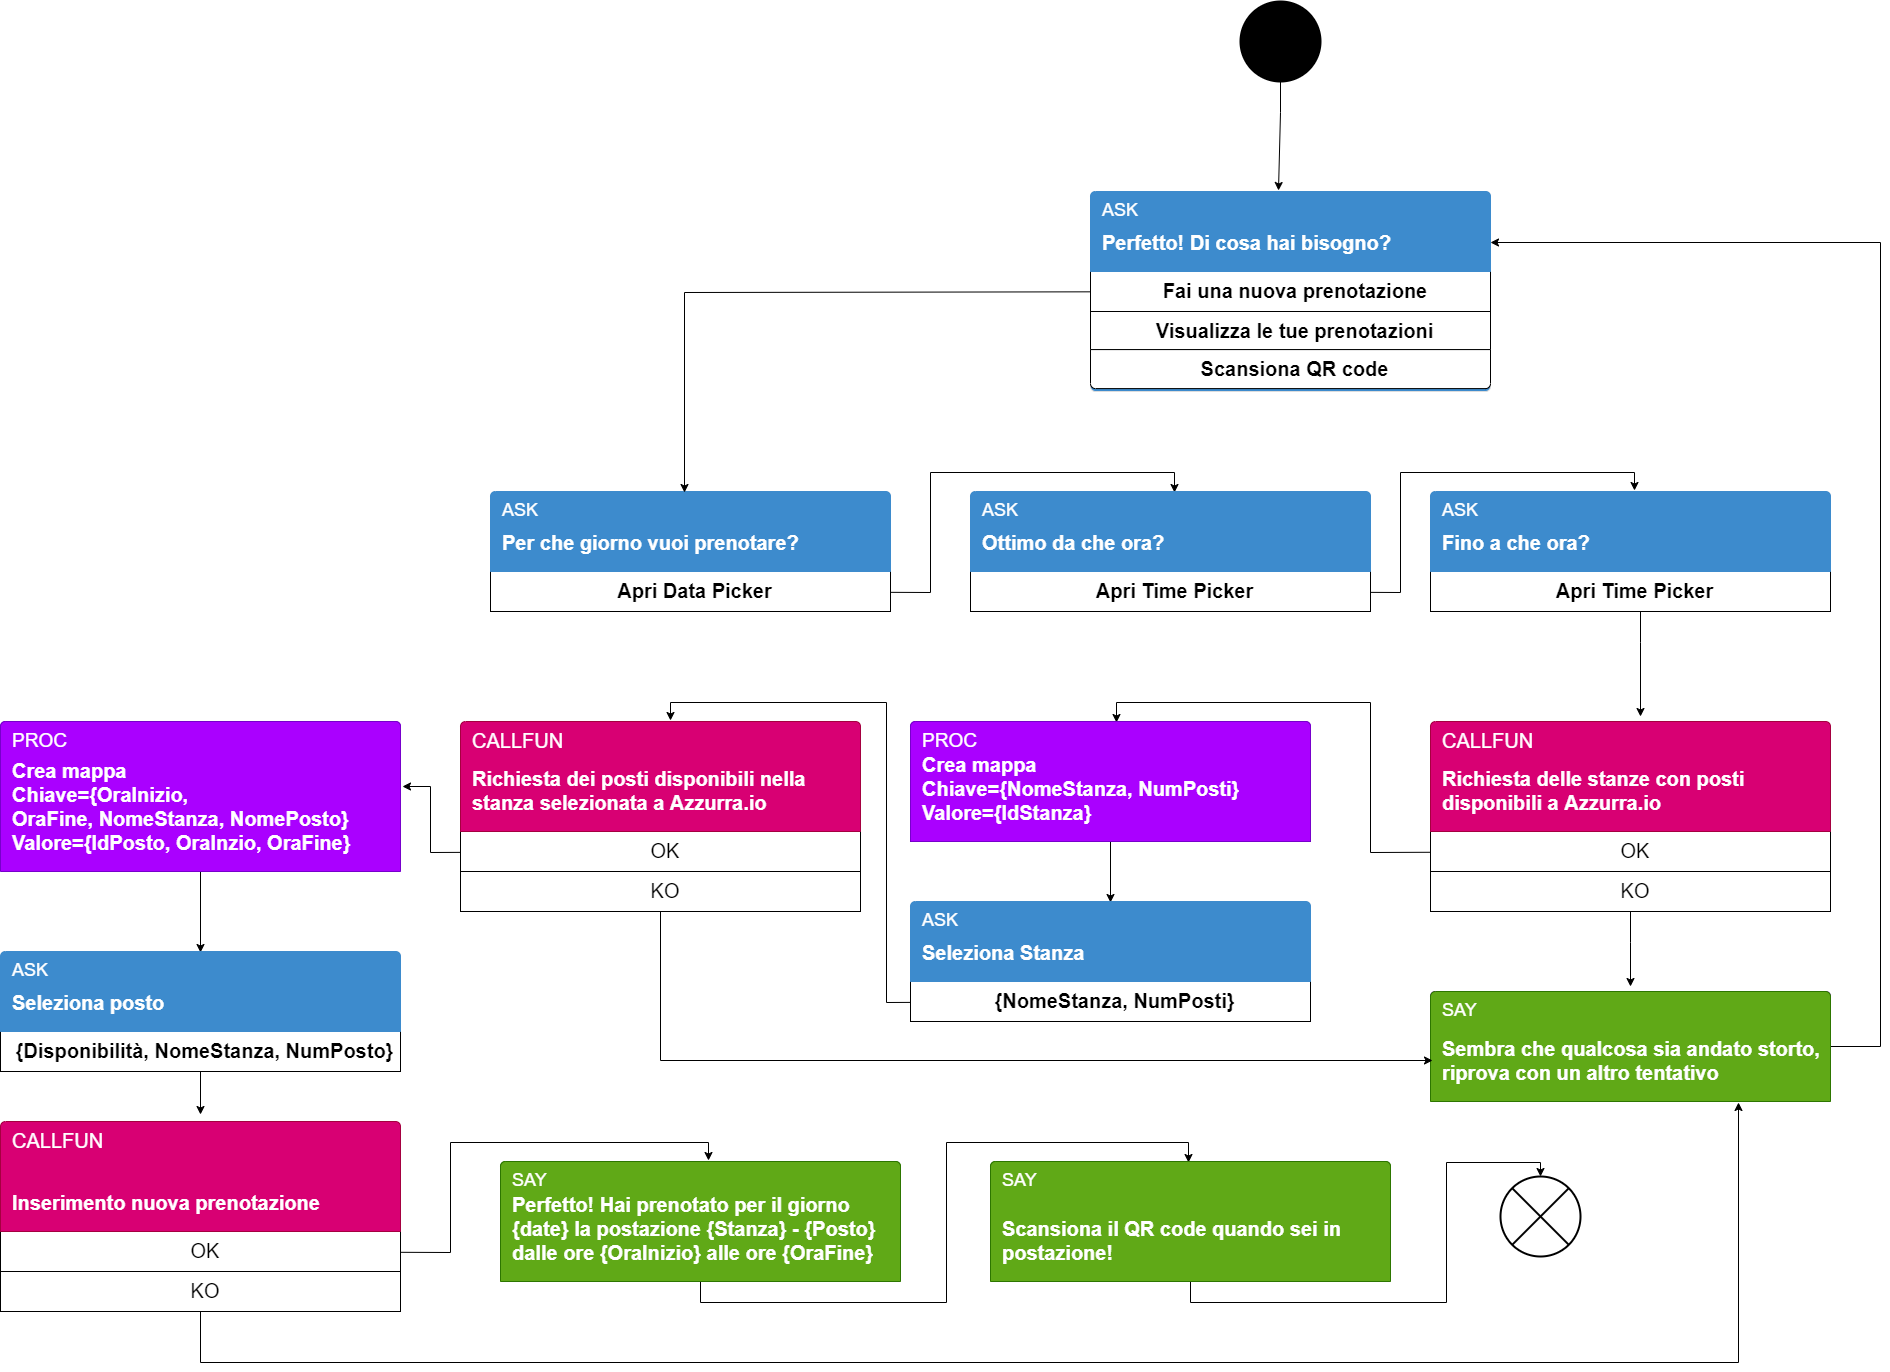
\includegraphics[scale=0.25]{chatbot/chatbot1.png}
	\caption{Diagramma per l'inserimento di una nuova prenotazione del flusso DeskBooking}\label{fig:ins}
\end{figure}

La Figura~\ref{fig:ins} rappresenta il ramo del flusso Deskbooking dedicato all'inserimento di una nuova prenotazione. È così composto:
\begin{enumerate}
	\item Il flusso inizia con un blocco ASK che chiede all'utente se vuole inserire una nuova prenotazione o scansionare un \g{QR code};
	\item Nel caso in cui l'utente voglia inserire una nuova prenotazione, attraverso un blocco ASK, viene chiesta la data che vuole inserire per la prenotazione. Viene progettato che l'inserimento della data viene fatta attraverso il DATEPICKER;
	\item Successivamente viene chiesta l'ora di inizio per la prenotazione tramite un blocco ASK. L'inserimento dell'ora avviene tramite il TIMEPICKER;
	\item Viene rifatta la stessa operazione del punto precedente ma chiedendo la data in cui finisce la prenotazione;
	\item Terminato il punto precedente, l'utente ha inserito l'intervallo di tempo all'interno del quale desidera effettuare una prenotazione di un posto a sedere. Attraverso il blocco CALLFUN viene chiesto ad Azzurra.io quali stanze con posti liberi sono disponibili per la data e l'intervallo inseriti dall'utente;
	\item Se non ci sono stanze con posti liberi o l'operazione di richiesta va in errore, attraverso un blocco SAY viene informato l'utente della situazione e ricomincia l'esecuzione dall'inizio del flusso;
	\item Se invece ci sono stanze con posti liberi, attraverso il blocco PROC vengono formattati i dati ricevuti in modo da poterli mostrare in una forma adatta alla situazione. In questo caso viene chiesto di creare una mappa con chiave contenente il nome della stanza e il numero dei posti e come valore l'identificativo della stanza. Quando si vorrà mostrare questi dati, verrà solo mostrato la chiave dei dati;
	\item Tramite il blocco ASK vengono mostrate le stanze disponibili mostrando i dati secondo la formattazione fatta al punto precedente;
	\item L'utente sceglie la stanza è viene controllato se nel frattempo è ancora disponibile e chiede quali posti a sedere sono liberi;
	\item Se avviene un errore di connessione o non ci sono più posti liberi si torna al punto 6 spiegato precedentemente;
	\item I dati ricevuti vengono formattati attraverso il blocco PROC creando la mappa con chiave contenente ora di inizio, orario di terminazione, nome stanza e nome posto a sedere, mentre come valore conterrà l'identificativo del posto a sedere, l'orario di inizio e di fine;
	\item Viene chiesto all'utente, attraverso un blocco ASK, di scegliere uno dei posti a sedere liberi;
	\item Viene contattato Azzurra.io con il blocco CALLFUN per inserire la nuova prenotazione;
	\item Se avviene un errore nell'inserimento viene eseguito il punto 6;
	\item Se l'operazione va a buon fine viene comunicato all'utente l'esito positivo dell'operazione, ricordandogli i dati della prenotazione e di scansionare il \g{QR code} per riscattare il posto a sedere. Il flusso poi termina.
\end{enumerate}

\begin{figure}[h]
	\centering
	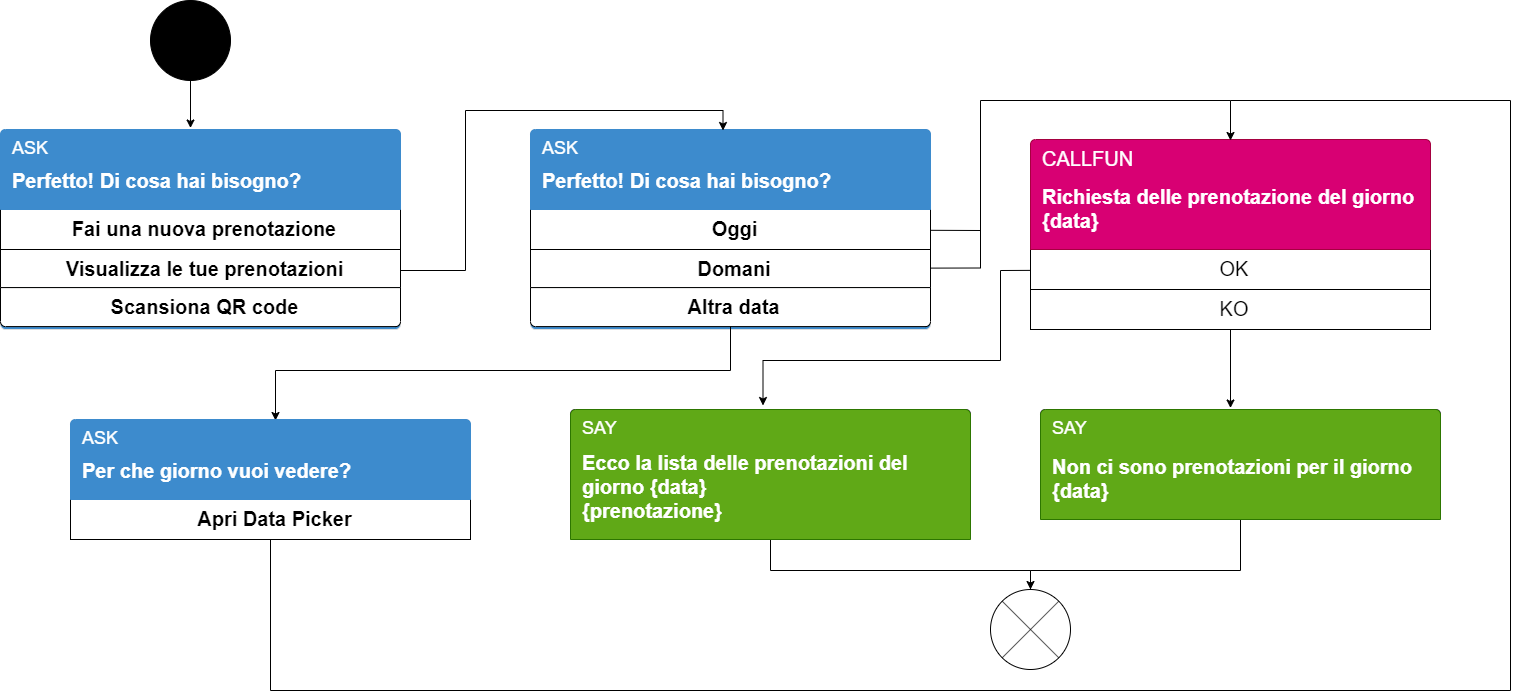
\includegraphics[scale=0.27]{chatbot/chatbot2.png}
	\caption{Diagramma per la visualizzazione delle prenotazioni del flusso DeskBooking}\label{fig:vis}
\end{figure}

La Figura~\ref{fig:vis} rappresenta il ramo del flusso Deskbooking dedicato alla visualizzazione delle prenotazioni. È così composto:
\begin{enumerate}
	\item Il flusso inizia con un blocco ASK che chiede all'utente se vuole inserire una nuova prenotazione o scansionare un \g{QR code};
	\item Nel caso in cui l'utente voglia visualizzare le sue prenotazioni, viene chiesto attraverso un blocco ASK se vuole sapere le prenotazione del giorno corrente o del giorno successivo o di un altro giorno;
	\item Nel caso l'utente voglia vedere le sue prenotazioni del giorno corrente o del giorno successivo verrà fatta una richiesta ad Azzurra.io per ottenere le prenotazioni della data inserita dall'utente. La richiesta viene fatta attraverso il blocco CALLFUN;
	\item Se invece l'utente vuole vedere le sue prenotazioni di una data diversa dal giorno corrente o successivo, attraverso un blocco ASK viene chiesta la data che vuole inserire per la visualizzazione. L'inserimento della data viene fatta attraverso il DATEPICKER, successivamente si esegue il punto 3 per la richiesta;
	\item Se ci sono prenotazioni queste vengono mostrate all'utente, se invece avviene un errore o non ci sono prenotazioni fatte da lui, verrà avvisato di tale evento. Dopo questo passo il flusso termina.\\
\end{enumerate}

\begin{figure}[h]
	\centering
	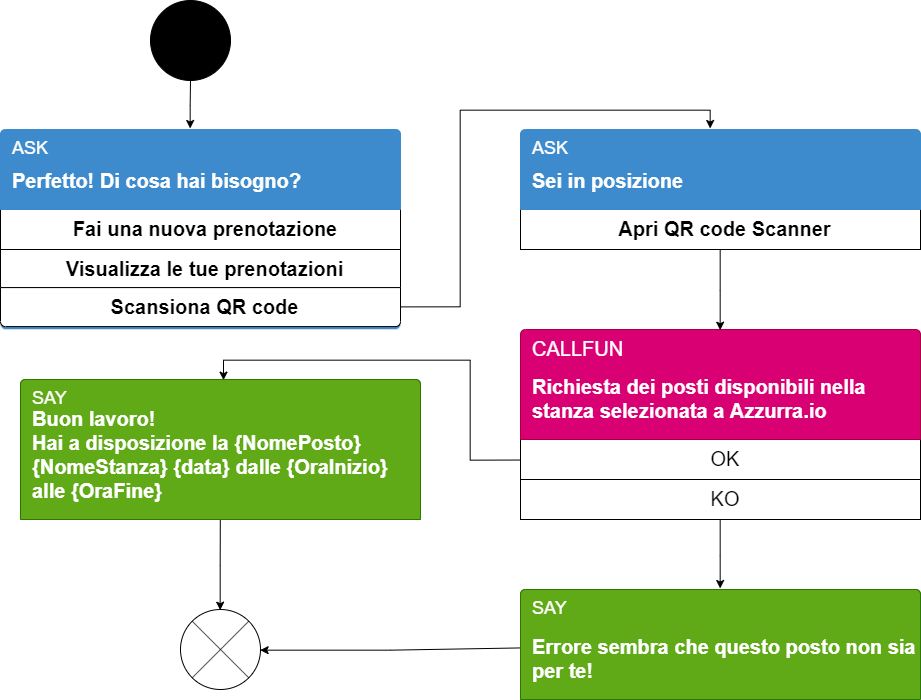
\includegraphics[scale=0.275]{chatbot/chatbot3.png}
	\caption{Diagramma per lo scansionamento del \g{QR code} del flusso DeskBooking}\label{fig:qrcode}
\end{figure}

La Figura~\ref{fig:qrcode} rappresenta il ramo del flusso Deskbooking dedicato allo scansionamento del \g{QR code}. È così composto:

\begin{enumerate}
	\item Il flusso inizia con un blocco ASK che chiede all'utente se vuole inserire una nuova prenotazione o scansionare un \g{QR code};
	\item Nel caso in cui l'utente voglia scansionare un \g{QR code} per riscattare il suo posto a sedere prenotato, viene chiesto attraverso un blocco ASK di aprire lo scannerizzatore di \g{QR code}. Viene usato QRSCANNER per leggere il \g{QR code};
	\item Viene chiesto ad Azzurra.io attraverso il blocco CALLFUN, se il posto a sedere può essere usato dall'utente;
	\item Se l'esito è positivo, viene comunicato all'utente che può usufruire del posto fino al termine della prenotazione. Termina così il flusso;
	\item Se l'esito è negativo, viene informato l'utente che non può usare il posto a sedere in quel momento. Termina così il flusso;
\end{enumerate}

\subsection{Visualizzazione della pianificazione}
Nel seguente diagramma viene mostrato l'insieme dei blocchi che fanno parte del flusso conversazionale Planning.

\begin{figure}[h]
	\centering
	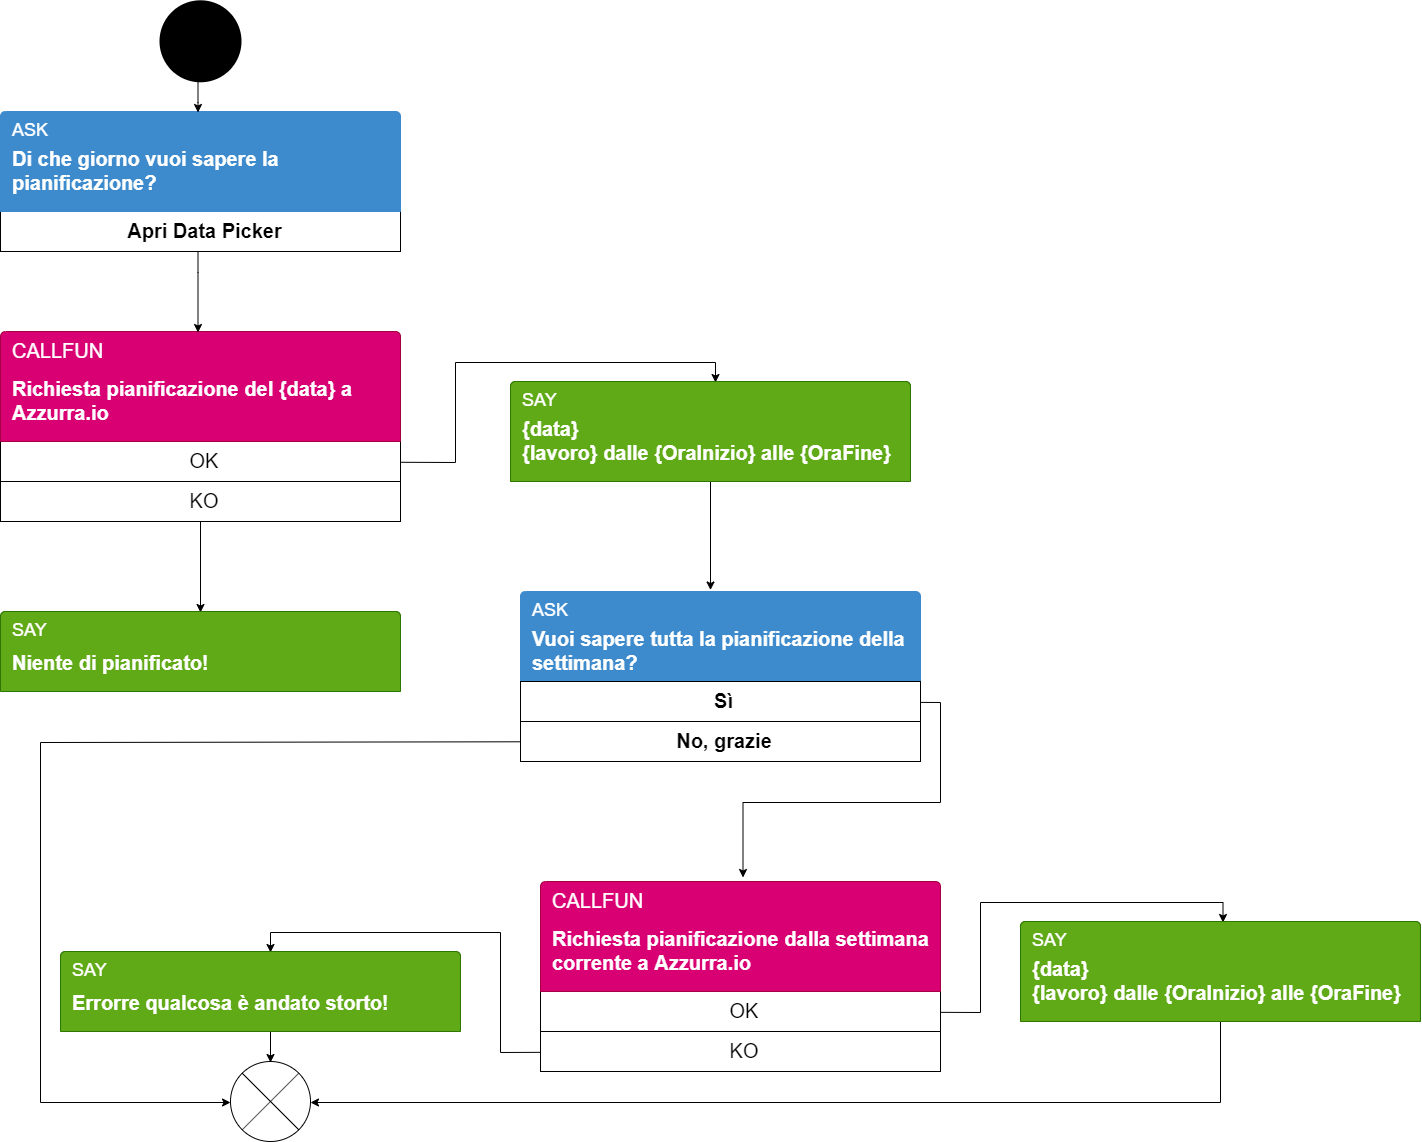
\includegraphics[scale=0.29]{chatbot/chatbot4.png}
	\caption{Diagramma per la visualizzazione della pianificazione del flusso Planning}\label{fig:plan}
\end{figure}

La Figura~\ref{fig:plan} rappresenta il ramo del flusso Planning dedicato alla visione della pianificazione del lavoro da svolgere.
\begin{enumerate}
	\item Il flusso inizia con un blocco ASK che chiede all'utente di quale giorno vuole vedere la pianificazione. L'inserimento della data viene fatta attraverso il DATEPICKER;
	\item Viene fatta richiesta a Azzurra.io, utilizzando il blocco CALLFUN, di trovare la pianificazione del giorno indicato dall'utente;
	\item Se non viene trovato nulla allora l'utente viene avvisato tramite un blocco SAY che non c'è niente di pianificato e il flusso termina;
	\item Se invece c'è una pianificazione disponibile per il giorno indicato dall'utente, viene visualizzata attraverso un blocco SAY;
	\item Dopo il punto precedentemente descritto viene chiesto con un blocco SAY se si vuole sapere la pianificazione di tutta la settimana;
	\item Se l'utente risponde no il flusso termina;
	\item Se l'utente risponde sì viene fatta richiesta a Azzurra.io, utilizzando il blocco CALLFUN, di trovare la pianificazione della settimana corrente;
	\item Se la richiesta va buon fine viene mostrata la pianificazione della settimana, altrimenti viene mostrato un messaggio. In entrambi i casi il flusso poi termina.
\end{enumerate}
\clearpage

\section{Codifica}
Per implementare i due flussi si sono utilizzati i \g{framework} Angular e Ionic. Grazie a Angular si è potuto strutturare un’applicazione web come una gerarchia di componenti quindi, attraverso il linguaggio TypeScript, si è gestita l'\emph{application logic} mentre con \gls{HTML} e \gls{CSS} si è gestita la \emph{presentation logic}. Purtroppo solo l'uso di Angular non basta per poter sviluppare un'applicazione \emph{mobile} infatti solo utilizzando Angular si può sviluppare una applicazione web. Si è quindi usato Cordova, un \g{framework} che permette di sviluppare un'applicazione \emph{mobile} multi-piattaforma e offre \g{api} per accedere alle funzionalità native del dispositivo, ad esempio la fotocamera. Cordova infatti incapsula l'applicazione web e la esegue localmente all’interno di un’\g{applicazione nativa} che può interagire con le funzionalità del dispositivo. Per sfruttare le funzionalità di Angular e di Cordova assieme, è stato usato il \g{framework} Ionic che permette di creare un ambiente integrato che semplifica lo sviluppo di applicazioni offrendo anche componenti grafiche ottimizzate per i dispositivi \emph{mobile}.\\

Per quanto riguarda la codifica, per prima cosa si è implementato una configurazione \g{JSON} per ogni flusso, dove si sono codificati i vari blocchi progettati, utilizzando la sintassi spiegata nel precedente capitolo. Una volta scritte le due configurazioni si è dovuto aggiornare il \emph{main flow} aggiungendo nel primo blocco che viene eseguito, cioè un blocco ASK dove viene chiesto che funzionalità si vuole eseguire, due BlockItem per indicare le due nuove funzionalità offerte dai due flussi prodotti. Oltre alle due nuove scelte, nel \emph{main flow} sono stati aggiunti due blocchi JUMP per permettere di mandare in esecuzione i due nuovi flussi quando l'utente ne richiede l'esecuzione, subito dopo la selezione della funzionalità desiderata da parte dell'utente.\\

Per poter creare i tre Widget, DATEPICKER, TIMEPICKER e QRSCANNER, nel createActions() ho aggiunto tre metodi per ognuno dei tre Widget, che vengono chiamati da createActions() in base al tipo di Widget da creare. In questi tre nuovi metodi viene impostato il testo che devono mostrare e nel caso dei DATEPICKER e TIMEPICKER viene impostato anche il formato del giorno e dell'ora. Per ognuno di questi metodi ho creato un metodo specifico per ogni Widget che si occupa della creazione e dell'apertura, in particolare per il metodo che crea il QRSCANNER, \_openQRcode(), viene utilizzato il ModalController di Ionic per creare la classe dove è definita l'interfaccia grafica e i metodi per il funzionamento di QRSCANNER. Il ModalController di Ionic permette di aprire una nuova finestra, sopra a quella corrente, per visualizzare la componente Ionic definita nella nuova finestra, in questo caso la classe che implementa il lettore di \g{QR code}. Una volta finito di usare la nuova finestra, essa viene chiusa e si ritorna alla finestra precedente che sarà nello stato precedente all'apertura della nuova finestra. Ho dovuto perciò implementare la classe che gestisce il lettore \g{QR code}, denominata CameraComponent, dove al suo interno richiama il \emph{plugin} di Cordova, QR Scanner. QR Scanner è un \g{api} che permette di accedere alla fotocamera del dispositivo e di scansionare i \g{QR code}. Vengono quindi definiti due metodi in CameraComponent, un metodo per l'apertura della fotocamera, la lettura del \g{QR code} e la chiusura della fotocamera che successivamente invia l'eventuale valore letto al ModalController. Nel CameraComponent viene definito anche il suo aspetto grafico mostrato nella Figura~\ref{fig:qrc}.\\
 
  Nel ChatComponent ho implementato il metodo \_initGenericQRCode() il quale aspetta di ricevere il valore letto dal lettore di \g{QR code} che richiama quindi il metodo sendReply() di AzzurraService per dare inizio al il processo di creazione del messaggio dell'utente umano spiegato nel capitolo precedente. \\
  
  Per quanto riguarda i metodi per il DATEPICKER e per il TIMEPICKER, essi sono molto simili a quelli per gestire il lettore \g{QR code}, con la differenza che i metodi analoghi a \_openQRcode(), \_openDatePicker() e \_openTimePicker(), non utilizzano il ModalComponent ma l'ion-datetime, una componente grafica offerta da Ionic che può essere configurato per chiedere una data oppure un intervallo temporale; il risultato viene mostrato nella Figura~\ref{fig:date} e nella Figura~\ref{fig:time}. Quindi in questi due metodi ho definito come si devono presentare i due \emph{picker} e quindi non c'è stato bisogno di un \emph{component} apposito che li gestisca come per il QRSCANNER. 
\section{Risultati}

Nella Figura~\ref{fig:planning} viene mostrata la \emph{chat} tra Azzurra e l'utente per la visualizzazione della pianificazione, sia per un singolo giorno (prima figura) sia per tutta la settimana (seconda figura).\\

\begin{figure}[h]
	\begin{center}
		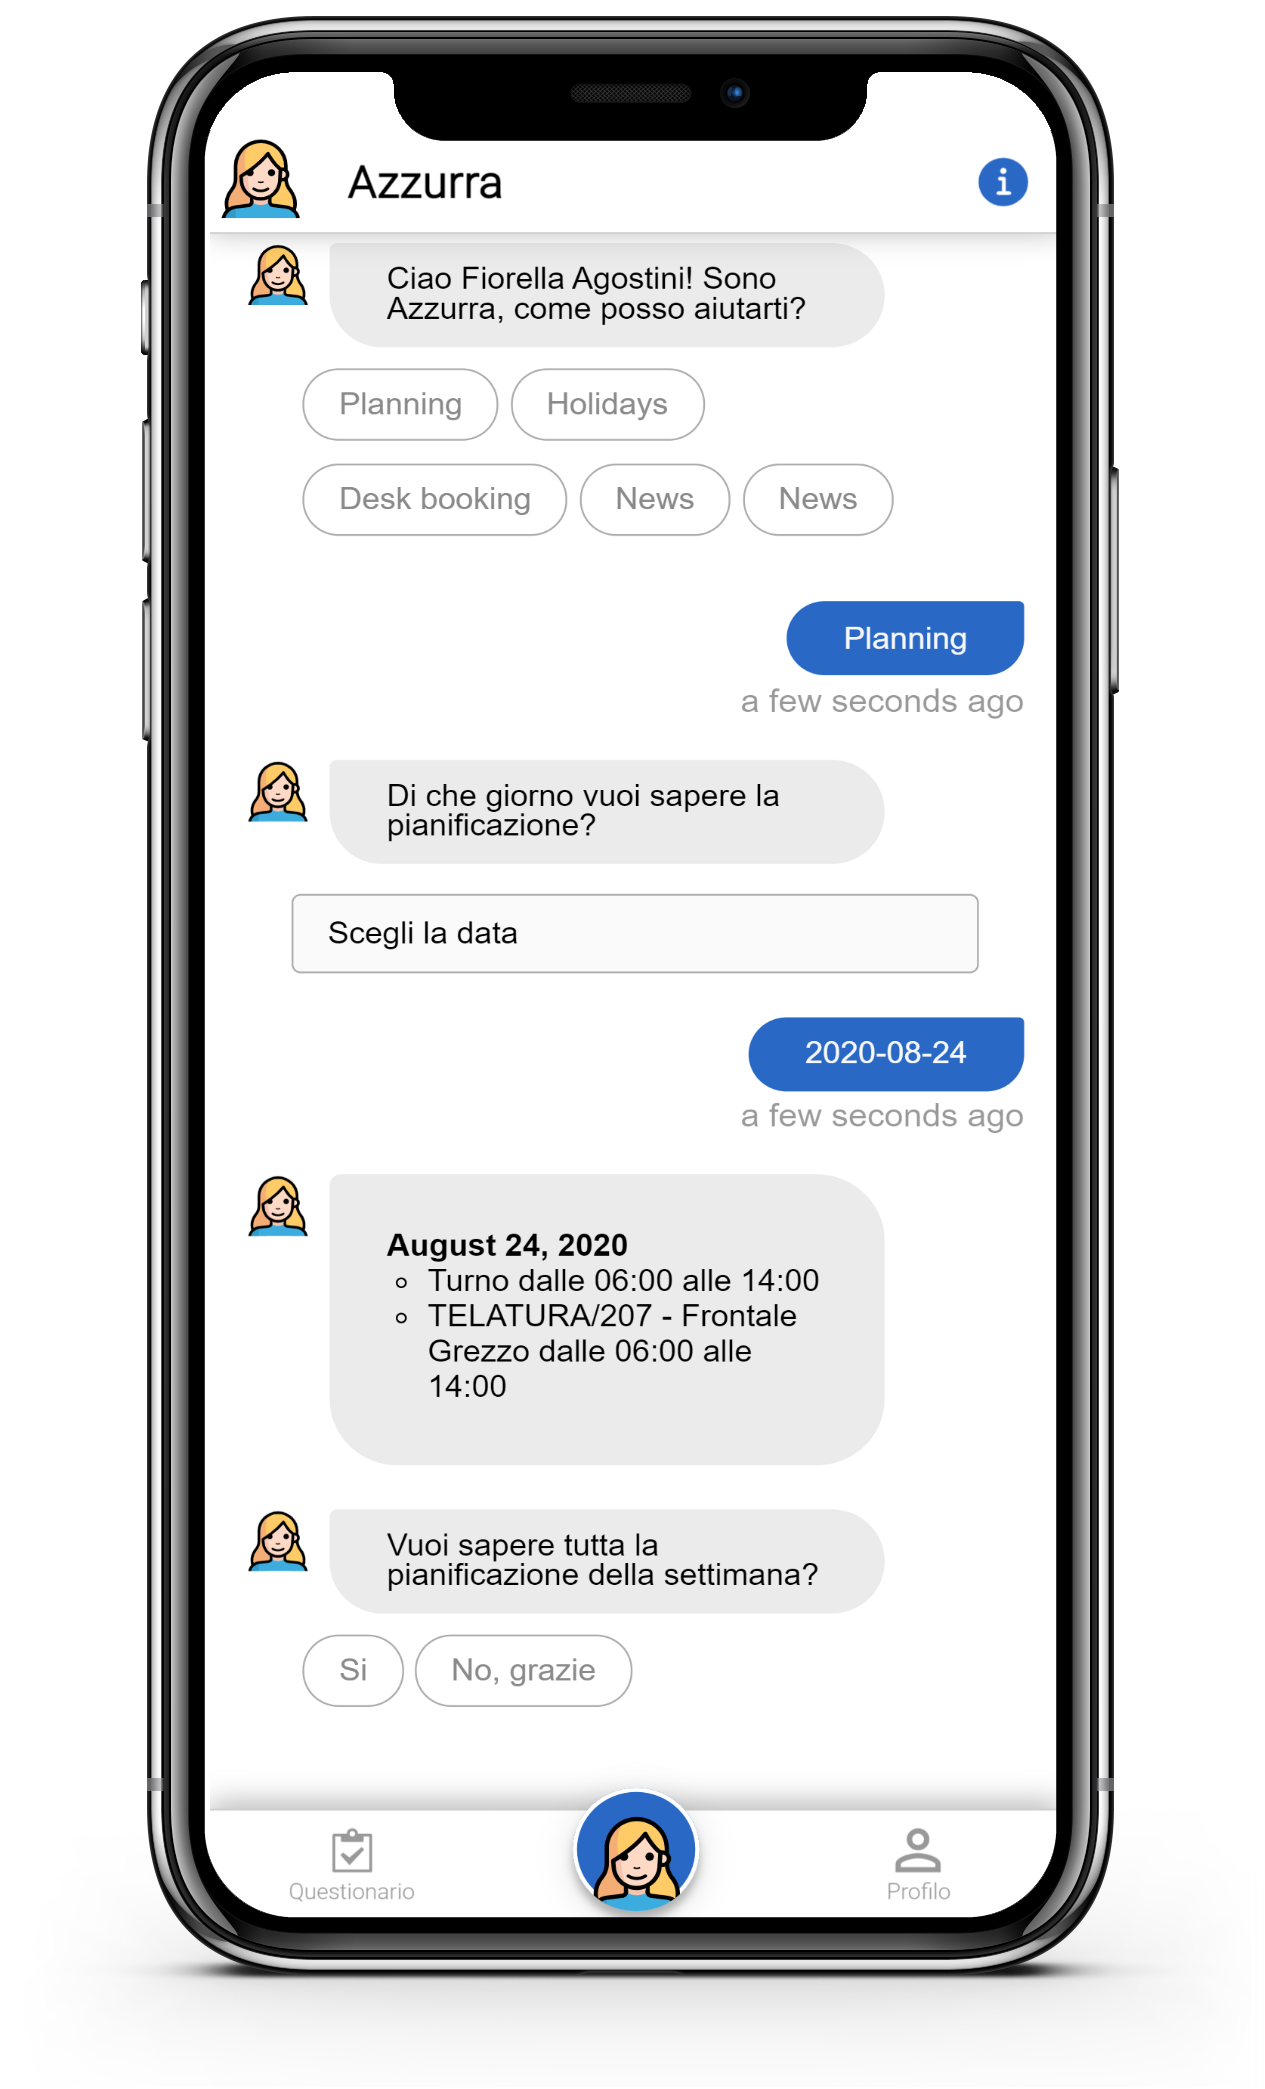
\includegraphics[scale=0.17]{day.png}\hfil
		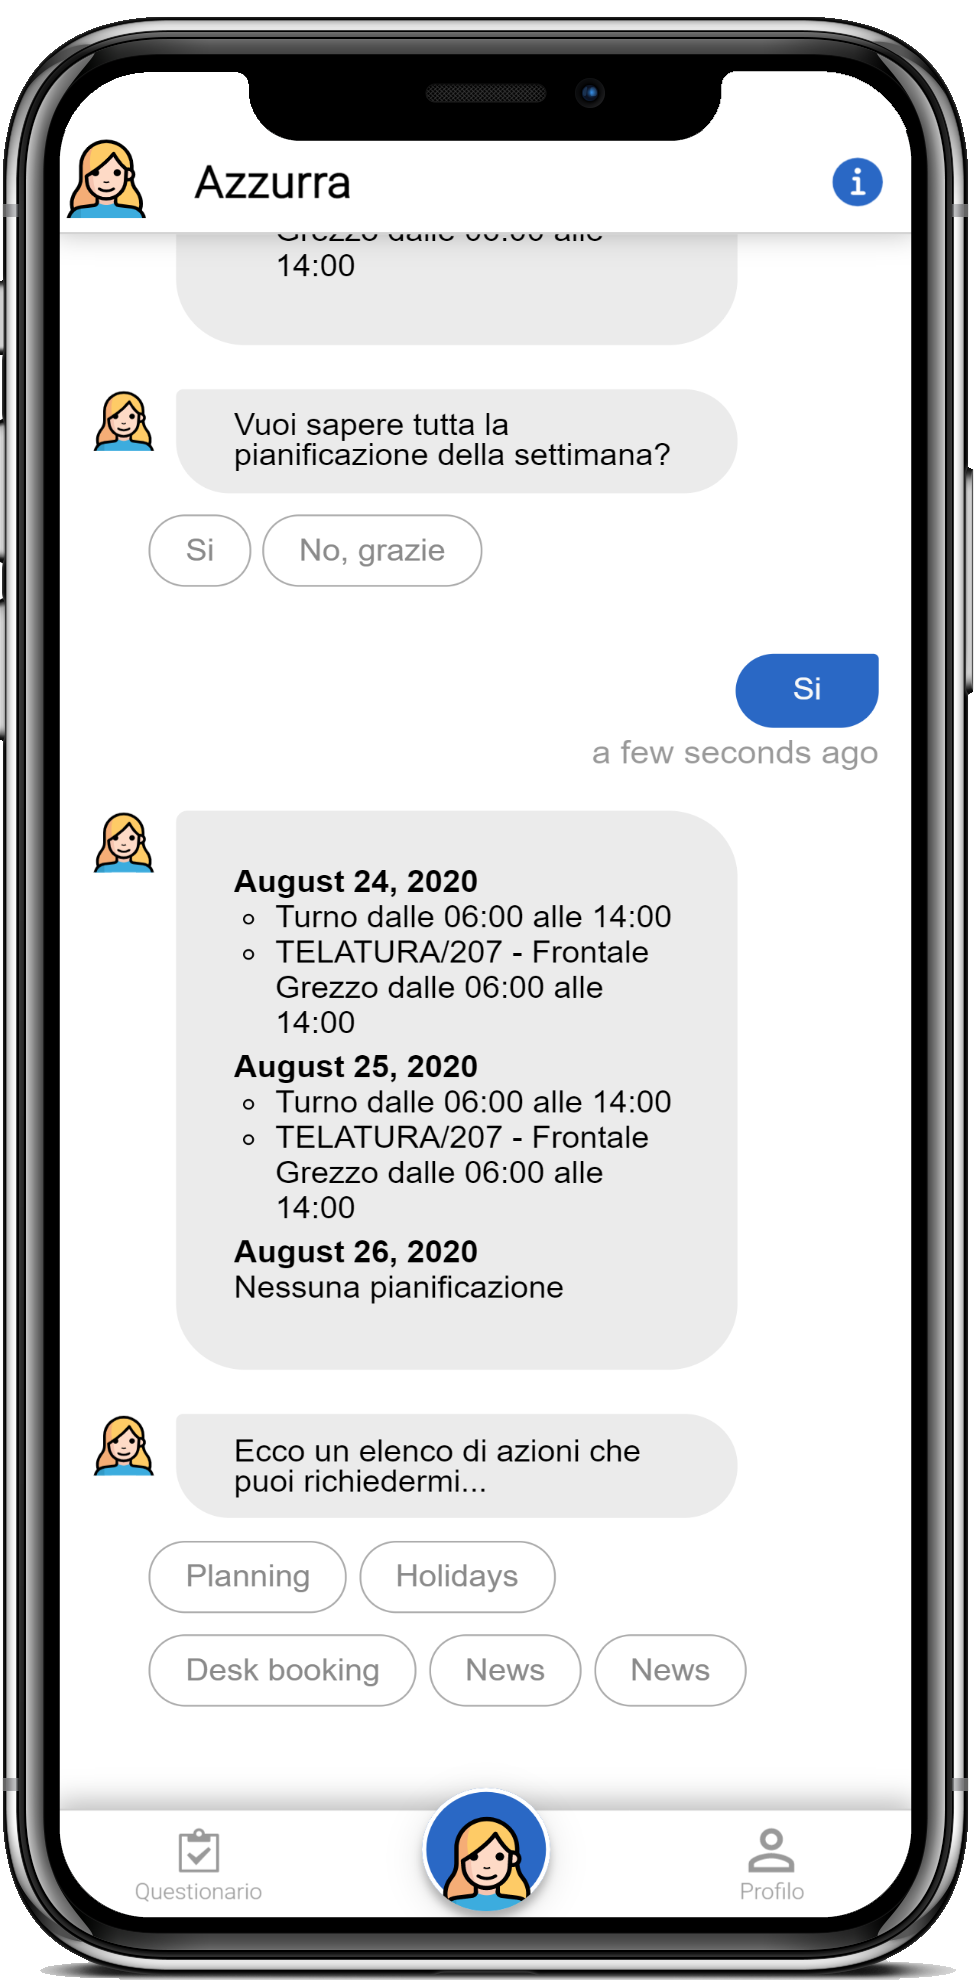
\includegraphics[scale=0.17]{week.png}
		\caption{Richiesta di visualizzazione della pianificazione}\label{fig:planning}
	\end{center}
\end{figure}

Nella Figura~\ref{fig:QRc} viene mostrata la \emph{chat} tra Azzurra e l'utente per la richiesta di visualizzazione del prenotazione dell'utente (prima figura) e la richiesta di scannerizzare il \g{QR code} per usufruire del posto prenotato (seconda figura).\\

\begin{figure}[h]
	\begin{center}
		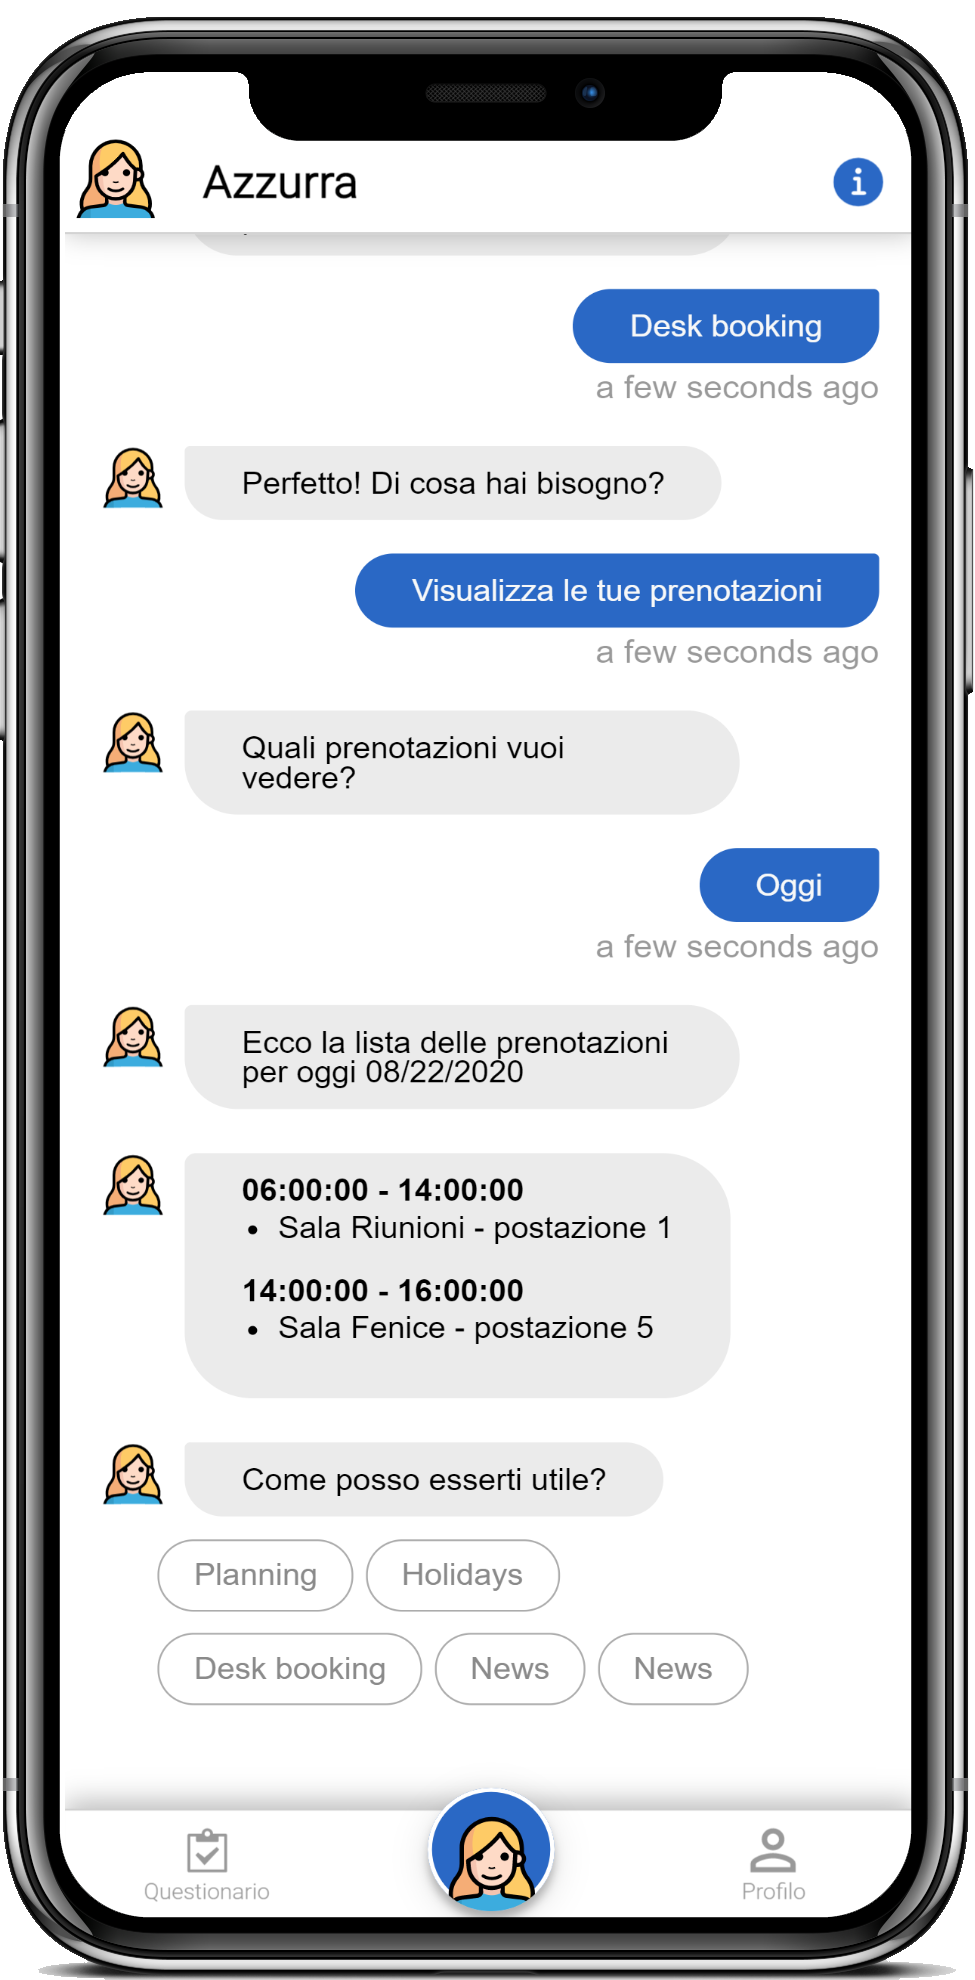
\includegraphics[scale=0.17]{visDB.png}\hfil
		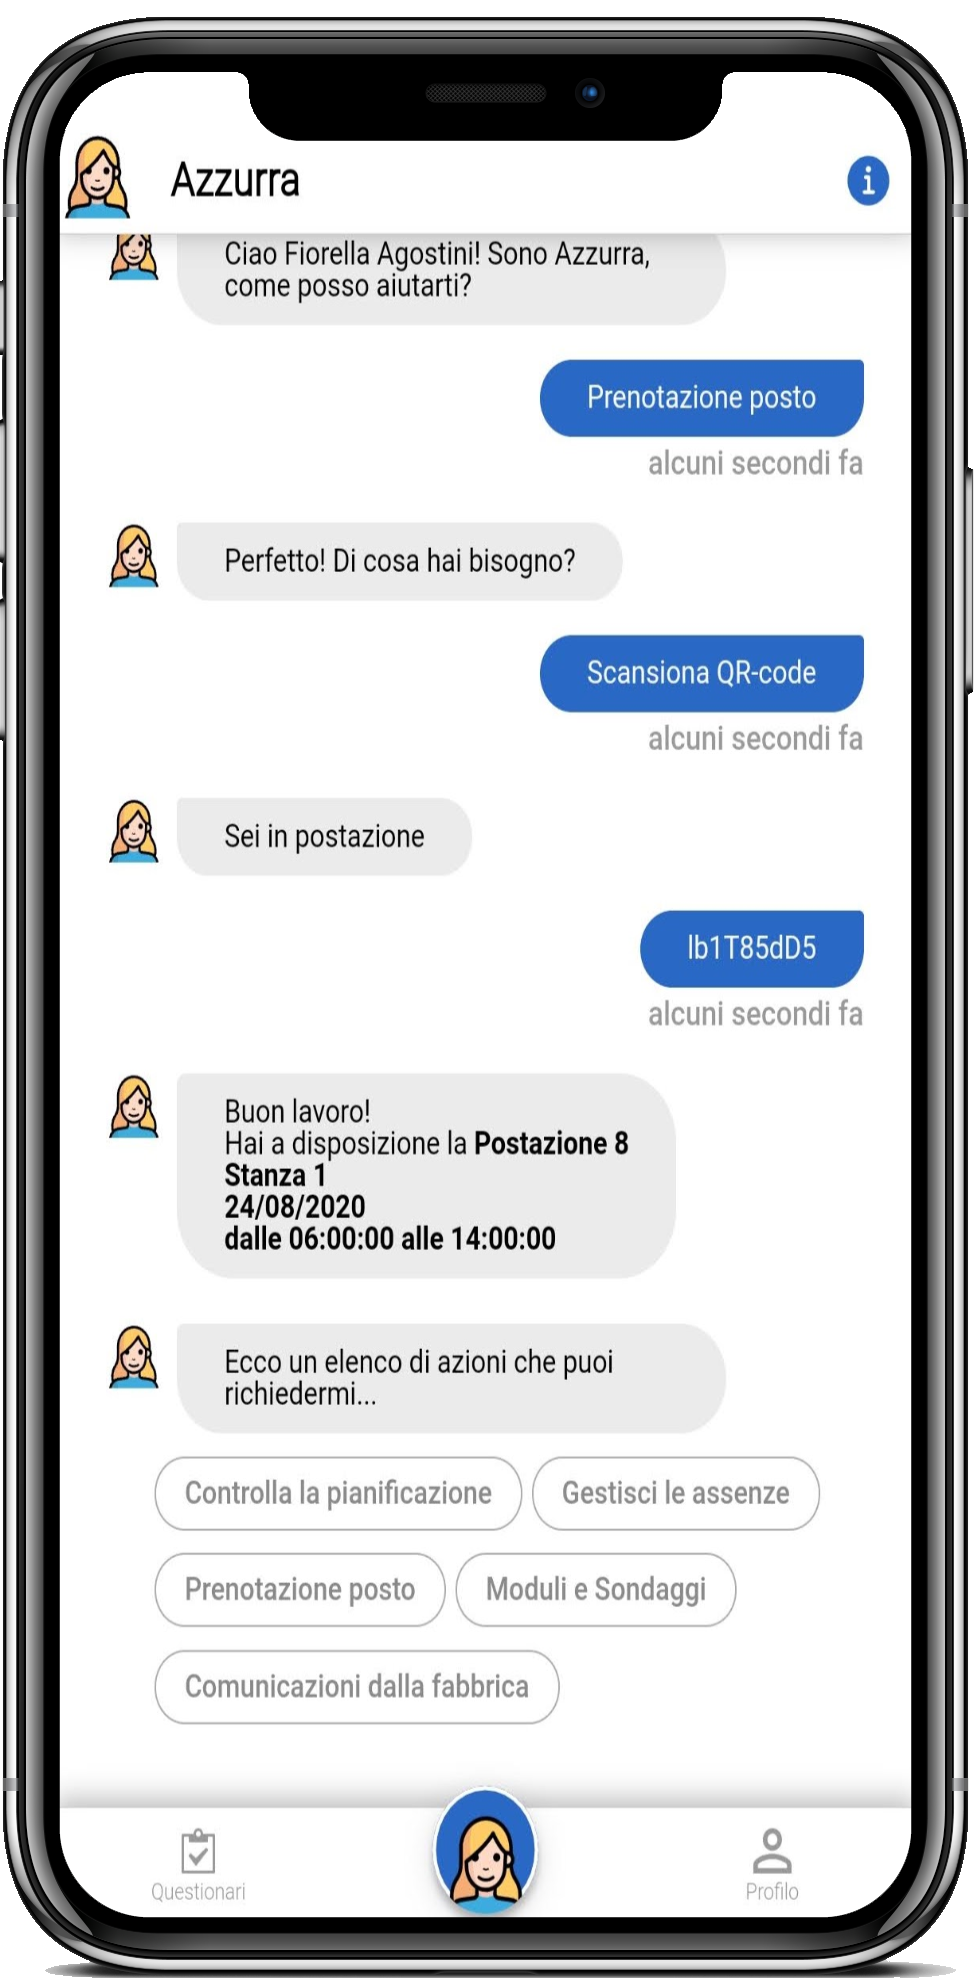
\includegraphics[scale=0.17]{qrc.png}
		\caption{Richiesta di visualizzazione delle prenotazioni e scannerizzazione di un QR code}\label{fig:QRc}
	\end{center}
\end{figure}

\begin{figure}[h]
	\begin{center}
		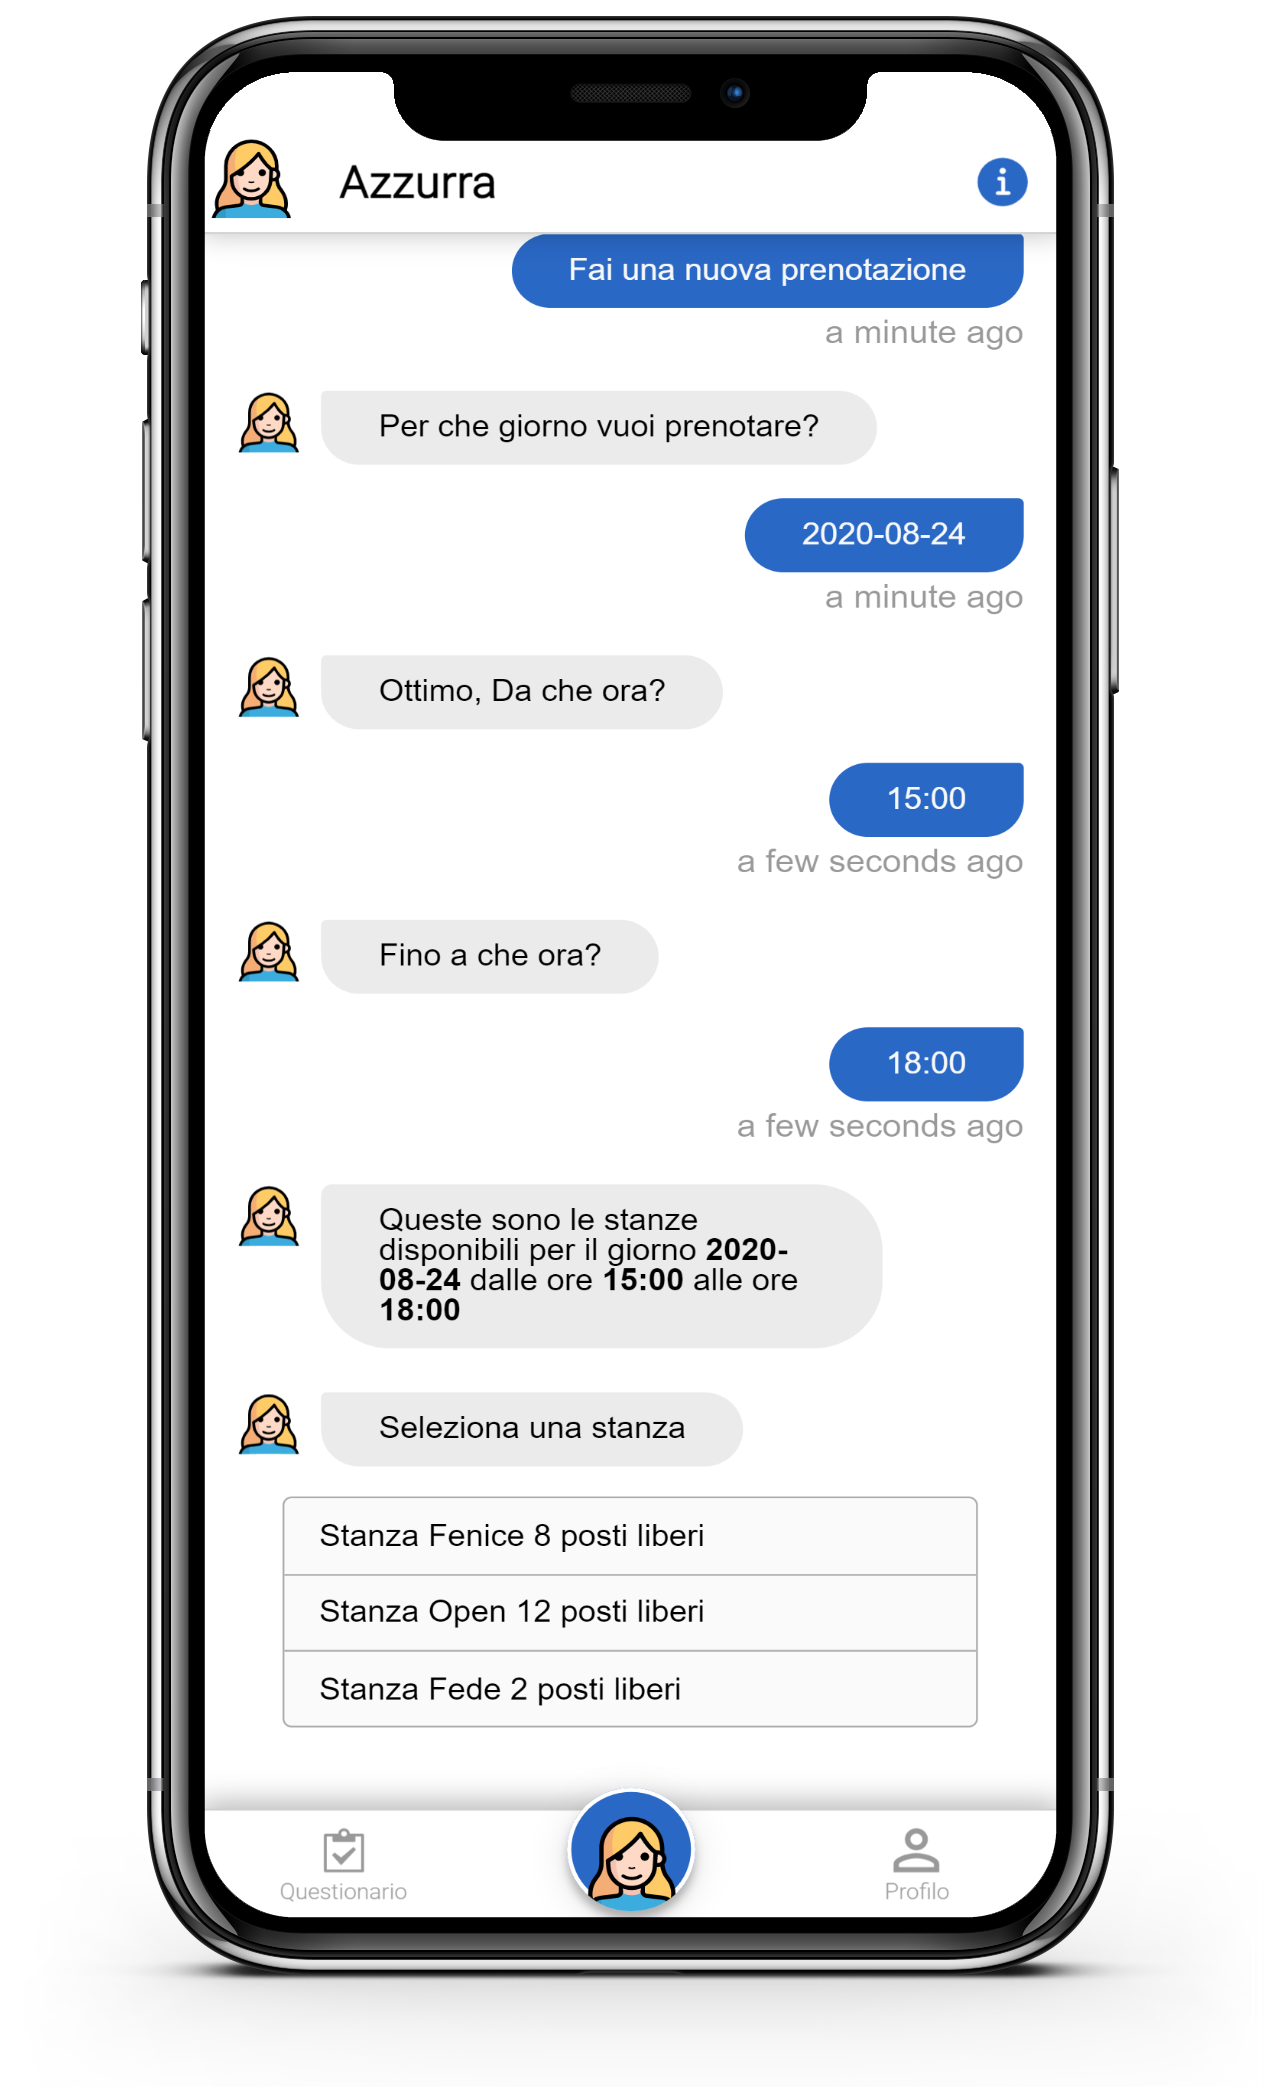
\includegraphics[scale=0.167]{DB1.png}\hfill
		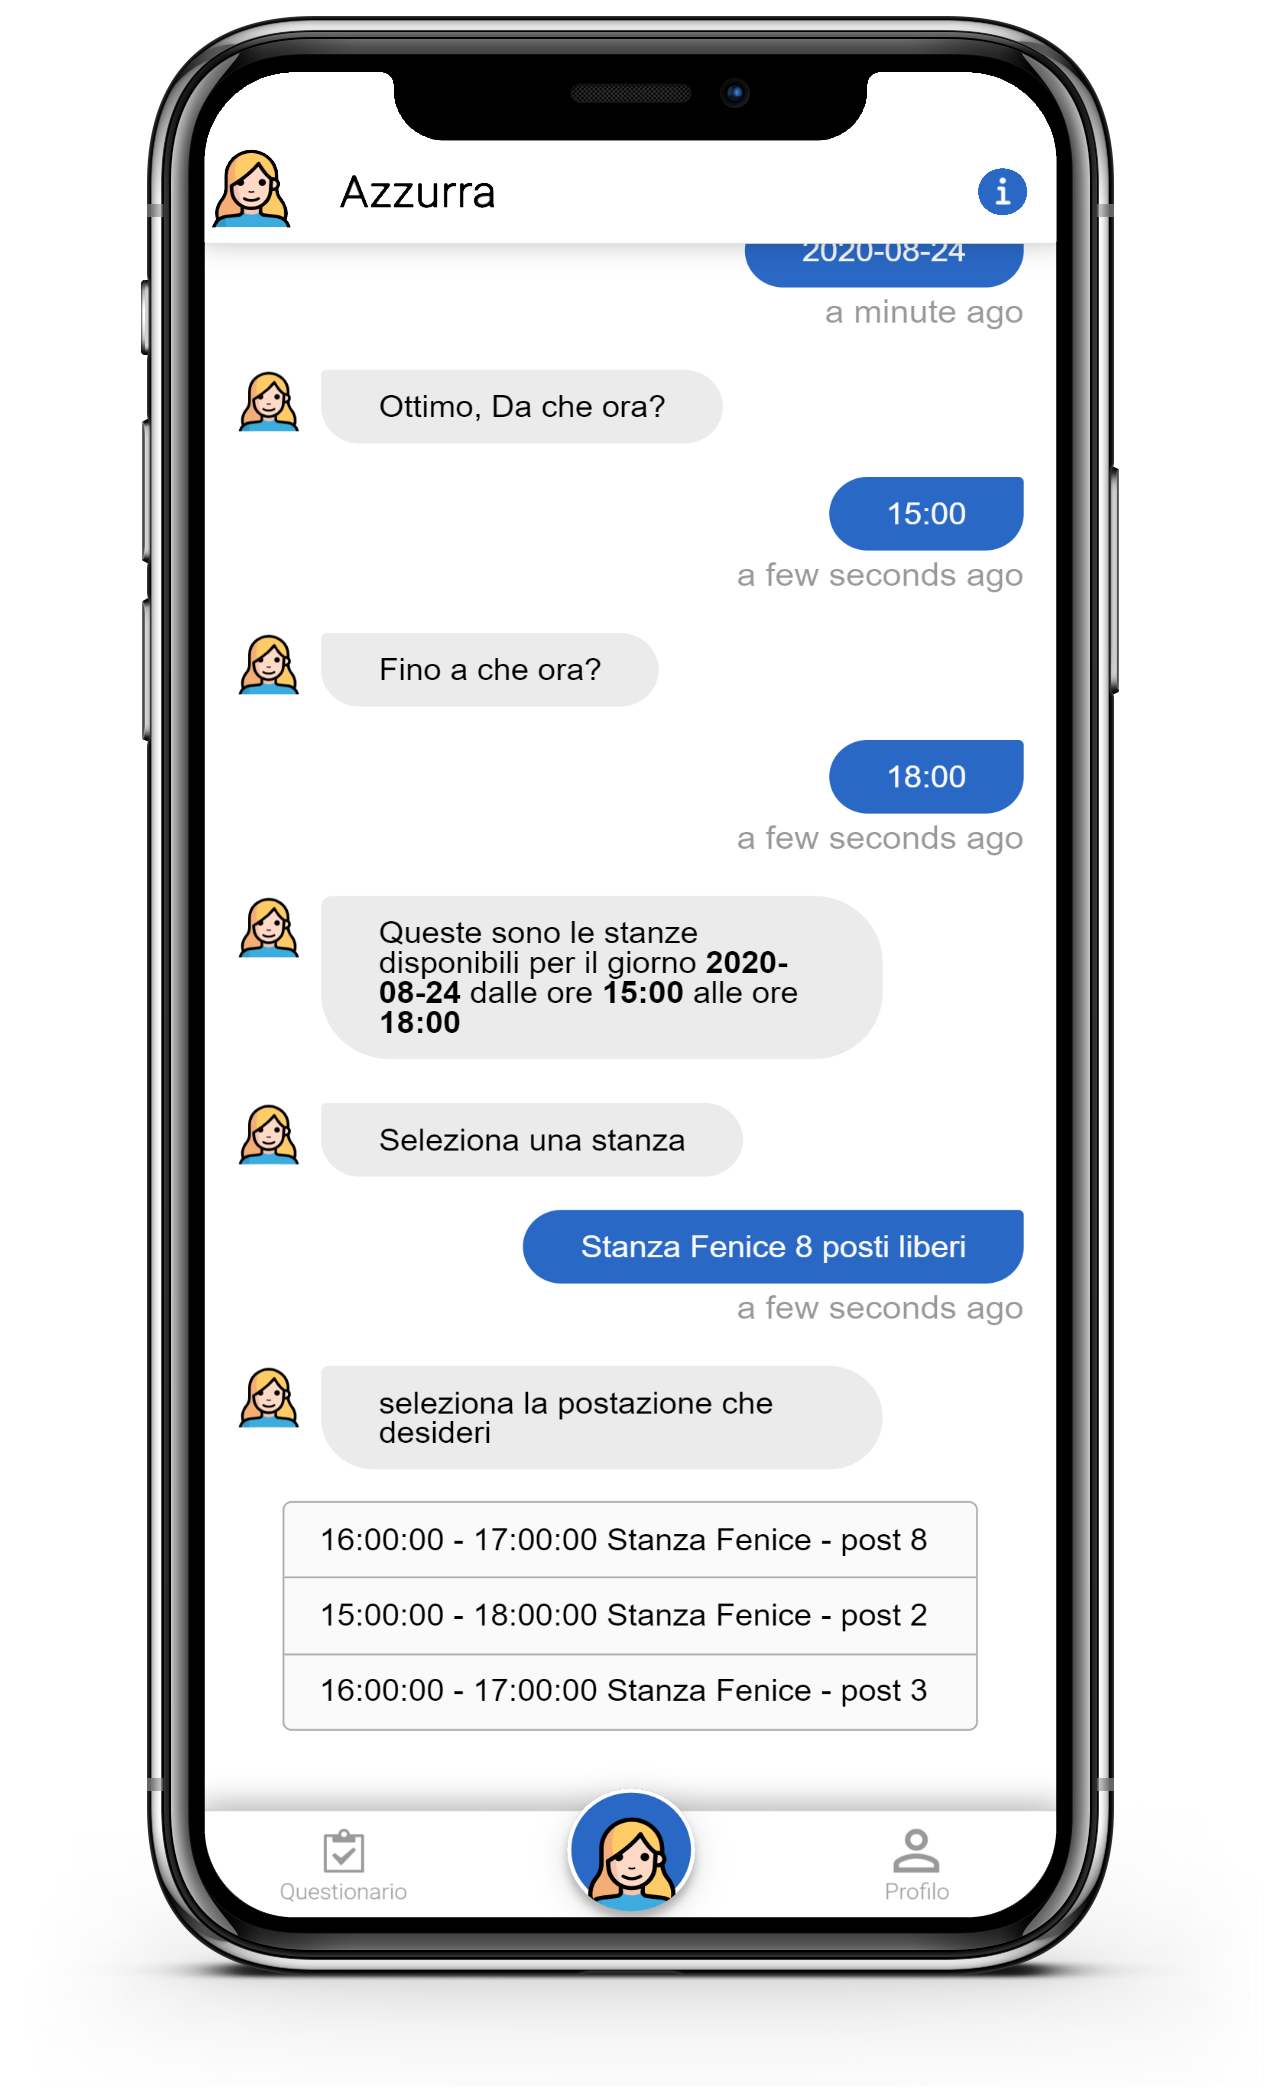
\includegraphics[scale=0.167]{DB2.png}\hfill
		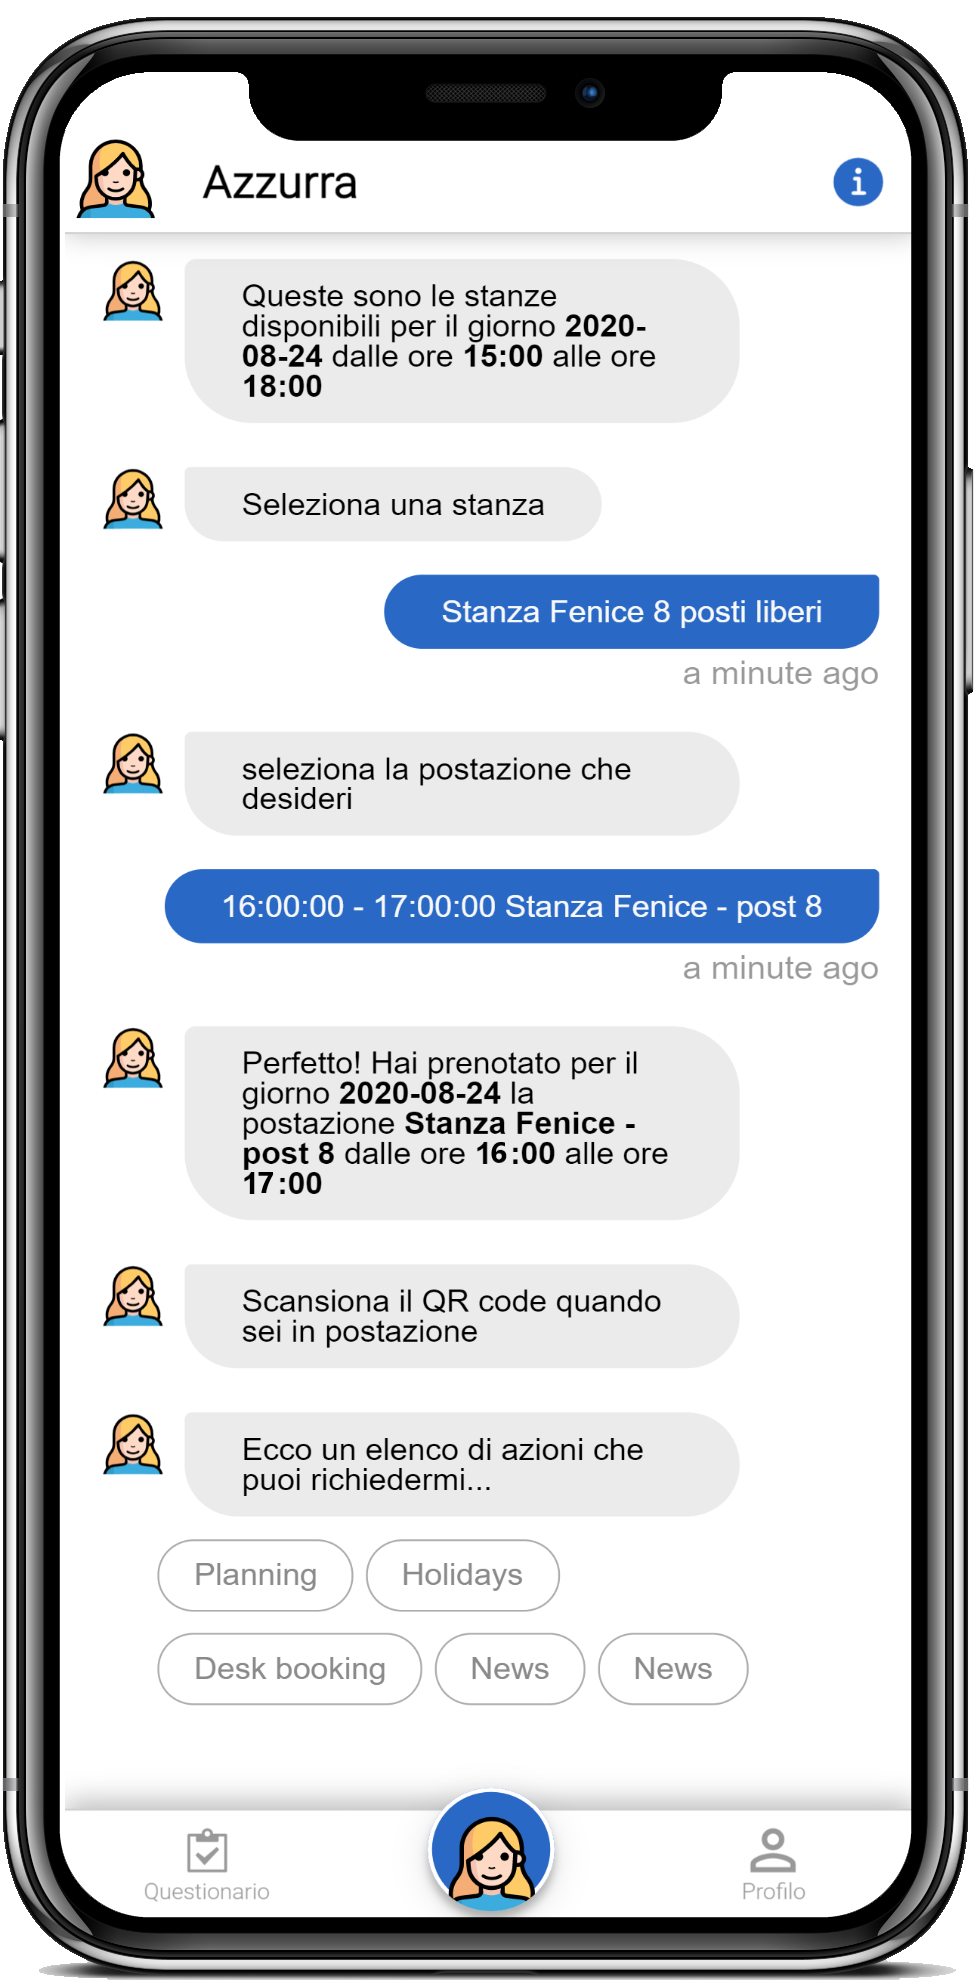
\includegraphics[scale=0.167]{DB3.png}
		\caption{Richiesta di inserimento di una nuova prenotazione}\label{fig:DB}
	\end{center}
\end{figure}
\clearpage
Nella Figura~\ref{fig:QRc} viene mostrata la \emph{chat} tra Azzurra e l'utente per la richiesta di inserimento di una nuova prenotazione. Viene perciò richiesto il giorno e l'intervallo di tempo in cui fare la prenotazione, in quale stanza deve essere il posto da prenotare e quale posto a sedere vuole prenotare tra quelli disponibili secondo i parametri inseriti.

\section{Considerazioni}
\label{cap:cons1}
I risultati ottenuti hanno soddisfatto tutti i requisiti stabili e sono stati soddisfacenti per il tutor aziendale. Dai risultati precedentemente elencati si sono fatte delle considerazioni su come potessero essere migliorati in termini di \emph{user experience}. L'\g{architettura} che supporta Azzurra permette di tenere lo storico dei messaggi e lo stato della conversazione per una certa durata, in modo da rendere migliore l'interazione tra utente e Azzurra. Un ulteriore miglioramento che può essere adottato è l'introduzione dei comandi vocali. Al momento l'inserimento dei dati da parte dell'utente avviene principalmente tramite comandi \emph{touch}. Talvolta questa interazione può risultare limitante per alcuni utenti ad esempio con limitazioni alla vista, all'uso delle mani o con il \emph{device} con schermo troppo piccolo. Grazie ai comandi vocali invece queste limitazioni risulterebbero annullate. \\

Dalla possibile introduzione dei comandi vocali nascono però altre considerazioni. Il riconoscimento vocale deve essere sufficientemente accurato da capire ciò che dice l'utente perché altrimenti può provocare una sensazione negativa di irritazione o frustrazione nell'utente dovuta al fatto che ciò che dice non viene capito dall'applicazione e quindi non offrire una buona \emph{user experience}. In sintesi, un possibile modo per migliorare l'\emph{user experience} è l'introduzione dei comandi vocali con un'accurata valutazione a priori di rischi e costi da affrontare.

